\documentclass[twoside]{book}

% Packages required by doxygen
\usepackage{calc}
\usepackage{doxygen}
\usepackage{graphicx}
\usepackage[utf8]{inputenc}
\usepackage{makeidx}
\usepackage{multicol}
\usepackage{multirow}
\usepackage{textcomp}
\usepackage[table]{xcolor}

% Font selection
\usepackage[T1]{fontenc}
\usepackage{mathptmx}
\usepackage[scaled=.90]{helvet}
\usepackage{courier}
\usepackage{amssymb}
\usepackage{sectsty}
\renewcommand{\familydefault}{\sfdefault}
\allsectionsfont{%
  \fontseries{bc}\selectfont%
  \color{darkgray}%
}
\renewcommand{\DoxyLabelFont}{%
  \fontseries{bc}\selectfont%
  \color{darkgray}%
}

% Page & text layout
\usepackage{geometry}
\geometry{%
  a4paper,%
  top=2.5cm,%
  bottom=2.5cm,%
  left=2.5cm,%
  right=2.5cm%
}
\tolerance=750
\hfuzz=15pt
\hbadness=750
\setlength{\emergencystretch}{15pt}
\setlength{\parindent}{0cm}
\setlength{\parskip}{0.2cm}
\makeatletter
\renewcommand{\paragraph}{%
  \@startsection{paragraph}{4}{0ex}{-1.0ex}{1.0ex}{%
    \normalfont\normalsize\bfseries\SS@parafont%
  }%
}
\renewcommand{\subparagraph}{%
  \@startsection{subparagraph}{5}{0ex}{-1.0ex}{1.0ex}{%
    \normalfont\normalsize\bfseries\SS@subparafont%
  }%
}
\makeatother

% Headers & footers
\usepackage{fancyhdr}
\pagestyle{fancyplain}
\fancyhead[LE]{\fancyplain{}{\bfseries\thepage}}
\fancyhead[CE]{\fancyplain{}{}}
\fancyhead[RE]{\fancyplain{}{\bfseries\leftmark}}
\fancyhead[LO]{\fancyplain{}{\bfseries\rightmark}}
\fancyhead[CO]{\fancyplain{}{}}
\fancyhead[RO]{\fancyplain{}{\bfseries\thepage}}
\fancyfoot[LE]{\fancyplain{}{}}
\fancyfoot[CE]{\fancyplain{}{}}
\fancyfoot[RE]{\fancyplain{}{\bfseries\scriptsize Generated on Wed Dec 4 2013 15\-:17\-:17 for my\-Tree by Doxygen }}
\fancyfoot[LO]{\fancyplain{}{\bfseries\scriptsize Generated on Wed Dec 4 2013 15\-:17\-:17 for my\-Tree by Doxygen }}
\fancyfoot[CO]{\fancyplain{}{}}
\fancyfoot[RO]{\fancyplain{}{}}
\renewcommand{\footrulewidth}{0.4pt}
\renewcommand{\chaptermark}[1]{%
  \markboth{#1}{}%
}
\renewcommand{\sectionmark}[1]{%
  \markright{\thesection\ #1}%
}

% Indices & bibliography
\usepackage{natbib}
\usepackage[titles]{tocloft}
\setcounter{tocdepth}{3}
\setcounter{secnumdepth}{5}
\makeindex

% Hyperlinks (required, but should be loaded last)
\usepackage{ifpdf}
\ifpdf
  \usepackage[pdftex,pagebackref=true]{hyperref}
\else
  \usepackage[ps2pdf,pagebackref=true]{hyperref}
\fi
\hypersetup{%
  colorlinks=true,%
  linkcolor=blue,%
  citecolor=blue,%
  unicode%
}

% Custom commands
\newcommand{\clearemptydoublepage}{%
  \newpage{\pagestyle{empty}\cleardoublepage}%
}


%===== C O N T E N T S =====

\begin{document}

% Titlepage & ToC
\hypersetup{pageanchor=false}
\pagenumbering{roman}
\begin{titlepage}
\vspace*{7cm}
\begin{center}%
{\Large my\-Tree \\[1ex]\large 0.\-1 }\\
\vspace*{1cm}
{\large Generated by Doxygen 1.8.5}\\
\vspace*{0.5cm}
{\small Wed Dec 4 2013 15:17:17}\\
\end{center}
\end{titlepage}
\clearemptydoublepage
\tableofcontents
\clearemptydoublepage
\pagenumbering{arabic}
\hypersetup{pageanchor=true}

%--- Begin generated contents ---
\chapter{Namespace Index}
\section{Namespace List}
Here is a list of all documented namespaces with brief descriptions\-:\begin{DoxyCompactList}
\item\contentsline{section}{\hyperlink{namespacecli}{cli} \\*Used for work with class Tree in C\-L\-I }{\pageref{namespacecli}}{}
\item\contentsline{section}{\hyperlink{namespacenode}{node} \\*Used for Node-\/relation classes }{\pageref{namespacenode}}{}
\item\contentsline{section}{\hyperlink{namespacetree}{tree} \\*Used for Tree-\/relation clasees }{\pageref{namespacetree}}{}
\end{DoxyCompactList}

\chapter{Hierarchical Index}
\section{Class Hierarchy}
This inheritance list is sorted roughly, but not completely, alphabetically\-:\begin{DoxyCompactList}
\item \contentsline{section}{tree\-:\-:Basic\-Error}{\pageref{classtree_1_1BasicError}}{}
\begin{DoxyCompactList}
\item \contentsline{section}{tree\-:\-:Address\-Error}{\pageref{classtree_1_1AddressError}}{}
\item \contentsline{section}{tree\-:\-:Insert\-Error}{\pageref{classtree_1_1InsertError}}{}
\end{DoxyCompactList}
\item \contentsline{section}{node\-:\-:Basic\-Error}{\pageref{classnode_1_1BasicError}}{}
\begin{DoxyCompactList}
\item \contentsline{section}{node\-:\-:Address\-Error}{\pageref{classnode_1_1AddressError}}{}
\item \contentsline{section}{node\-:\-:Insert\-Error}{\pageref{classnode_1_1InsertError}}{}
\end{DoxyCompactList}
\item \contentsline{section}{node\-:\-:Node}{\pageref{classnode_1_1Node}}{}
\item \contentsline{section}{tree\-:\-:Tree}{\pageref{classtree_1_1Tree}}{}
\end{DoxyCompactList}

\chapter{Class Index}
\section{Class List}
Here are the classes, structs, unions and interfaces with brief descriptions\-:\begin{DoxyCompactList}
\item\contentsline{section}{\hyperlink{classnode_1_1AddressError}{node\-::\-Address\-Error} \\*Thrown if try to access empty place }{\pageref{classnode_1_1AddressError}}{}
\item\contentsline{section}{\hyperlink{classtree_1_1AddressError}{tree\-::\-Address\-Error} \\*Thrown if try to access empty place }{\pageref{classtree_1_1AddressError}}{}
\item\contentsline{section}{\hyperlink{classtree_1_1BasicError}{tree\-::\-Basic\-Error} \\*Basic error class }{\pageref{classtree_1_1BasicError}}{}
\item\contentsline{section}{\hyperlink{classnode_1_1BasicError}{node\-::\-Basic\-Error} \\*Basic error class }{\pageref{classnode_1_1BasicError}}{}
\item\contentsline{section}{\hyperlink{classnode_1_1InsertError}{node\-::\-Insert\-Error} \\*Thrown if try to add node to busy place }{\pageref{classnode_1_1InsertError}}{}
\item\contentsline{section}{\hyperlink{classtree_1_1InsertError}{tree\-::\-Insert\-Error} \\*Thrown if try to add something to busy place }{\pageref{classtree_1_1InsertError}}{}
\item\contentsline{section}{\hyperlink{classnode_1_1Node}{node\-::\-Node} \\*This class provides atomized operations relationed to current node }{\pageref{classnode_1_1Node}}{}
\item\contentsline{section}{\hyperlink{classtree_1_1Tree}{tree\-::\-Tree} \\*Used for encapsulate \hyperlink{classnode_1_1Node}{node\-::\-Node} structures }{\pageref{classtree_1_1Tree}}{}
\end{DoxyCompactList}

\chapter{Namespace Documentation}
\hypertarget{namespacecli}{\section{cli Namespace Reference}
\label{namespacecli}\index{cli@{cli}}
}


Used for work with class Tree in C\-L\-I.  


\subsection*{Functions}
\begin{DoxyCompactItemize}
\item 
\hypertarget{namespacecli_af03ae5779bc6d1ef6ea0d26e052e5ead}{void \hyperlink{namespacecli_af03ae5779bc6d1ef6ea0d26e052e5ead}{clear} ()}\label{namespacecli_af03ae5779bc6d1ef6ea0d26e052e5ead}

\begin{DoxyCompactList}\small\item\em Clears input stream. \end{DoxyCompactList}\item 
\hypertarget{namespacecli_a532bad7ea5db107b523244fcac93aaef}{void \hyperlink{namespacecli_a532bad7ea5db107b523244fcac93aaef}{print\-Use\-Msg} ()}\label{namespacecli_a532bad7ea5db107b523244fcac93aaef}

\begin{DoxyCompactList}\small\item\em Prints basic usage message. \end{DoxyCompactList}\item 
\hypertarget{namespacecli_a773376d1405b7896ded70368022ca7c6}{void \hyperlink{namespacecli_a773376d1405b7896ded70368022ca7c6}{print\-Help\-Msg} ()}\label{namespacecli_a773376d1405b7896ded70368022ca7c6}

\begin{DoxyCompactList}\small\item\em Prints help message. \end{DoxyCompactList}\item 
\hypertarget{namespacecli_a99771d2f58982bc684fc57765e964538}{std\-::string \hyperlink{namespacecli_a99771d2f58982bc684fc57765e964538}{input\-Name} ()}\label{namespacecli_a99771d2f58982bc684fc57765e964538}

\begin{DoxyCompactList}\small\item\em Gets and process strings (may be with spaces) from input stream. \end{DoxyCompactList}\item 
bool \hyperlink{namespacecli_af6d116280d09587b4754e10973a9aee3}{choose\-Branch} ()
\begin{DoxyCompactList}\small\item\em Process user selection of tree branch to use. \end{DoxyCompactList}\end{DoxyCompactItemize}


\subsection{Detailed Description}
Used for work with class Tree in C\-L\-I. 

\subsection{Function Documentation}
\hypertarget{namespacecli_af6d116280d09587b4754e10973a9aee3}{\index{cli@{cli}!choose\-Branch@{choose\-Branch}}
\index{choose\-Branch@{choose\-Branch}!cli@{cli}}
\subsubsection[{choose\-Branch}]{\setlength{\rightskip}{0pt plus 5cm}bool cli\-::choose\-Branch (
\begin{DoxyParamCaption}
{}
\end{DoxyParamCaption}
)}}\label{namespacecli_af6d116280d09587b4754e10973a9aee3}


Process user selection of tree branch to use. 

User may select left(default) or right branch. Returns 1 if right selected; 0 in other way. 

Definition at line 57 of file cli.\-hpp.


\hypertarget{namespacenode}{\section{node Namespace Reference}
\label{namespacenode}\index{node@{node}}
}


Used for Node-\/relation classes.  


\subsection*{Classes}
\begin{DoxyCompactItemize}
\item 
class \hyperlink{classnode_1_1BasicError}{Basic\-Error}
\begin{DoxyCompactList}\small\item\em Basic error class. \end{DoxyCompactList}\item 
class \hyperlink{classnode_1_1InsertError}{Insert\-Error}
\begin{DoxyCompactList}\small\item\em Thrown if try to add node to busy place. \end{DoxyCompactList}\item 
class \hyperlink{classnode_1_1AddressError}{Address\-Error}
\begin{DoxyCompactList}\small\item\em Thrown if try to access empty place. \end{DoxyCompactList}\item 
class \hyperlink{classnode_1_1Node}{Node}
\begin{DoxyCompactList}\small\item\em This class provides atomized operations relationed to current node. \end{DoxyCompactList}\end{DoxyCompactItemize}
\subsection*{Functions}
\begin{DoxyCompactItemize}
\item 
\hypertarget{namespacenode_a3a207588fdbfd347567a11ed3d4004f1}{std\-::ostream \& \hyperlink{namespacenode_a3a207588fdbfd347567a11ed3d4004f1}{operator$<$$<$} (std\-::ostream \&os, const \hyperlink{classnode_1_1Node}{node\-::\-Node} \&c\-Node)}\label{namespacenode_a3a207588fdbfd347567a11ed3d4004f1}

\begin{DoxyCompactList}\small\item\em Outputs name of current node to output stream. \end{DoxyCompactList}\item 
void \hyperlink{namespacenode_abc231d3793b070782e2f2f74a9f8b7dd}{\-\_\-connect} (\hyperlink{classnode_1_1Node}{Node} $\ast$c\-Node, const \hyperlink{classnode_1_1Node}{Node} $\ast$p\-Node)
\begin{DoxyCompactList}\small\item\em Set pointer to parent of current node to selected node. \end{DoxyCompactList}\end{DoxyCompactItemize}


\subsection{Detailed Description}
Used for Node-\/relation classes. 

\subsection{Function Documentation}
\hypertarget{namespacenode_abc231d3793b070782e2f2f74a9f8b7dd}{\index{node@{node}!\-\_\-connect@{\-\_\-connect}}
\index{\-\_\-connect@{\-\_\-connect}!node@{node}}
\subsubsection[{\-\_\-connect}]{\setlength{\rightskip}{0pt plus 5cm}void node\-::\-\_\-connect (
\begin{DoxyParamCaption}
\item[{Node $\ast$}]{c\-Node, }
\item[{const Node $\ast$}]{p\-Node}
\end{DoxyParamCaption}
)}}\label{namespacenode_abc231d3793b070782e2f2f74a9f8b7dd}


Set pointer to parent of current node to selected node. 


\begin{DoxyParams}{Parameters}
{\em c\-Node} & -- current \hyperlink{classnode_1_1Node}{Node} \\
\hline
{\em p\-Node} & -- parent \hyperlink{classnode_1_1Node}{Node} \\
\hline
\end{DoxyParams}


Definition at line 415 of file node.\-hpp.


\hypertarget{namespacetree}{\section{tree Namespace Reference}
\label{namespacetree}\index{tree@{tree}}
}


Used for Tree-\/relation clasees.  


\subsection*{Classes}
\begin{DoxyCompactItemize}
\item 
class \hyperlink{classtree_1_1BasicError}{Basic\-Error}
\begin{DoxyCompactList}\small\item\em Basic error class. \end{DoxyCompactList}\item 
class \hyperlink{classtree_1_1InsertError}{Insert\-Error}
\begin{DoxyCompactList}\small\item\em Thrown if try to add something to busy place. \end{DoxyCompactList}\item 
class \hyperlink{classtree_1_1AddressError}{Address\-Error}
\begin{DoxyCompactList}\small\item\em Thrown if try to access empty place. \end{DoxyCompactList}\item 
class \hyperlink{classtree_1_1Tree}{Tree}
\begin{DoxyCompactList}\small\item\em Used for encapsulate \hyperlink{classnode_1_1Node}{node\-::\-Node} structures. \end{DoxyCompactList}\end{DoxyCompactItemize}
\subsection*{Typedefs}
\begin{DoxyCompactItemize}
\item 
\hypertarget{namespacetree_a36da3b38ad98fe87c16c4336cd5b8a44}{typedef std\-::vector$<$ std\-::string $>$ \hyperlink{namespacetree_a36da3b38ad98fe87c16c4336cd5b8a44}{Tree\-Nodes}}\label{namespacetree_a36da3b38ad98fe87c16c4336cd5b8a44}

\begin{DoxyCompactList}\small\item\em Vector of node content. \end{DoxyCompactList}\item 
\hypertarget{namespacetree_a1906ab31086935949f162ea3e2c41200}{typedef std\-::vector$<$ \hyperlink{namespacetree_a36da3b38ad98fe87c16c4336cd5b8a44}{Tree\-Nodes} $>$ \hyperlink{namespacetree_a1906ab31086935949f162ea3e2c41200}{Tree\-Content}}\label{namespacetree_a1906ab31086935949f162ea3e2c41200}

\begin{DoxyCompactList}\small\item\em Provides pretty tree representation. \end{DoxyCompactList}\end{DoxyCompactItemize}
\subsection*{Functions}
\begin{DoxyCompactItemize}
\item 
\hypertarget{namespacetree_a866148b74626a75c48e2b1228e2e455c}{std\-::ostream \& {\bfseries operator$<$$<$} (std\-::ostream \&os, const \hyperlink{classtree_1_1Tree}{tree\-::\-Tree} \&c\-Tree)}\label{namespacetree_a866148b74626a75c48e2b1228e2e455c}

\item 
\hypertarget{namespacetree_a674f9624f1c01eabd2eb8177740ca377}{std\-::ostream \& {\bfseries operator$<$$<$} (std\-::ostream \&os, const \hyperlink{classtree_1_1InsertError}{Insert\-Error} \&e)}\label{namespacetree_a674f9624f1c01eabd2eb8177740ca377}

\item 
\hypertarget{namespacetree_a3dec862cb2578d085095490c9a2dfee9}{std\-::ostream \& {\bfseries operator$<$$<$} (std\-::ostream \&os, const \hyperlink{classtree_1_1AddressError}{Address\-Error} \&e)}\label{namespacetree_a3dec862cb2578d085095490c9a2dfee9}

\end{DoxyCompactItemize}


\subsection{Detailed Description}
Used for Tree-\/relation clasees. 
\chapter{Class Documentation}
\hypertarget{classnode_1_1AddressError}{\section{node\-:\-:Address\-Error Class Reference}
\label{classnode_1_1AddressError}\index{node\-::\-Address\-Error@{node\-::\-Address\-Error}}
}


Thrown if try to access empty place.  




{\ttfamily \#include $<$node.\-hpp$>$}

Inheritance diagram for node\-:\-:Address\-Error\-:\begin{figure}[H]
\begin{center}
\leavevmode
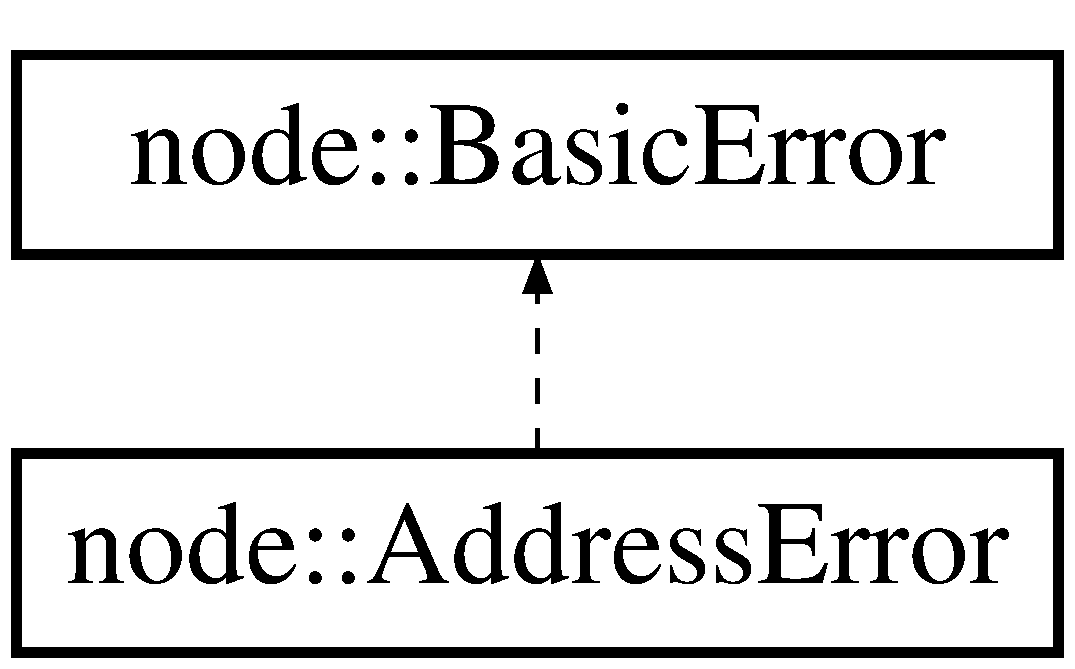
\includegraphics[height=2.000000cm]{classnode_1_1AddressError}
\end{center}
\end{figure}
\subsection*{Public Member Functions}
\begin{DoxyCompactItemize}
\item 
\hypertarget{classnode_1_1AddressError_ac65a406163e7de2536cbf9c401a69fd8}{{\bfseries Address\-Error} (const \hyperlink{classnode_1_1Node}{Node} $\ast$const i\-Pointer=N\-U\-L\-L)}\label{classnode_1_1AddressError_ac65a406163e7de2536cbf9c401a69fd8}

\item 
\hypertarget{classnode_1_1AddressError_aee194bc336a02d1cbd36a4d53b569f5c}{std\-::ostream \& {\bfseries operator$<$$<$} (std\-::ostream \&os)}\label{classnode_1_1AddressError_aee194bc336a02d1cbd36a4d53b569f5c}

\end{DoxyCompactItemize}
\subsection*{Additional Inherited Members}


\subsection{Detailed Description}
Thrown if try to access empty place. 

Definition at line 35 of file node.\-hpp.



The documentation for this class was generated from the following file\-:\begin{DoxyCompactItemize}
\item 
src/node.\-hpp\end{DoxyCompactItemize}

\hypertarget{classtree_1_1AddressError}{\section{tree\-:\-:Address\-Error Class Reference}
\label{classtree_1_1AddressError}\index{tree\-::\-Address\-Error@{tree\-::\-Address\-Error}}
}


Thrown if try to access empty place.  




{\ttfamily \#include $<$tree.\-hpp$>$}

Inheritance diagram for tree\-:\-:Address\-Error\-:\begin{figure}[H]
\begin{center}
\leavevmode
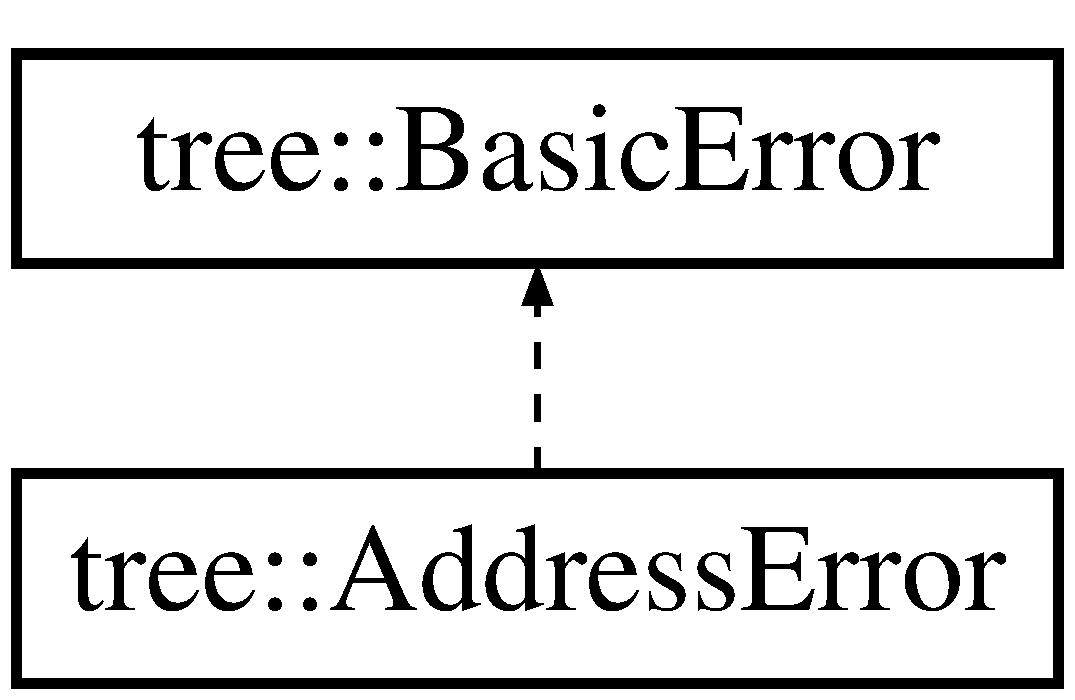
\includegraphics[height=2.000000cm]{classtree_1_1AddressError}
\end{center}
\end{figure}
\subsection*{Public Member Functions}
\begin{DoxyCompactItemize}
\item 
\hypertarget{classtree_1_1AddressError_a7aab83b45916e564f655344d25e5ebca}{{\bfseries Address\-Error} (const \hyperlink{classnode_1_1Node}{node\-::\-Node} $\ast$const i\-Pointer=N\-U\-L\-L)}\label{classtree_1_1AddressError_a7aab83b45916e564f655344d25e5ebca}

\end{DoxyCompactItemize}
\subsection*{Friends}
\begin{DoxyCompactItemize}
\item 
\hypertarget{classtree_1_1AddressError_a979849bdcb8ad88734190c5e012c1cff}{std\-::ostream \& {\bfseries operator$<$$<$} (std\-::ostream \&os, const \hyperlink{classtree_1_1AddressError}{Address\-Error} \&e)}\label{classtree_1_1AddressError_a979849bdcb8ad88734190c5e012c1cff}

\end{DoxyCompactItemize}
\subsection*{Additional Inherited Members}


\subsection{Detailed Description}
Thrown if try to access empty place. 

Definition at line 36 of file tree.\-hpp.



The documentation for this class was generated from the following file\-:\begin{DoxyCompactItemize}
\item 
src/tree.\-hpp\end{DoxyCompactItemize}

\hypertarget{classtree_1_1BasicError}{\section{tree\-:\-:Basic\-Error Class Reference}
\label{classtree_1_1BasicError}\index{tree\-::\-Basic\-Error@{tree\-::\-Basic\-Error}}
}


Basic error class.  




{\ttfamily \#include $<$tree.\-hpp$>$}

Inheritance diagram for tree\-:\-:Basic\-Error\-:\begin{figure}[H]
\begin{center}
\leavevmode
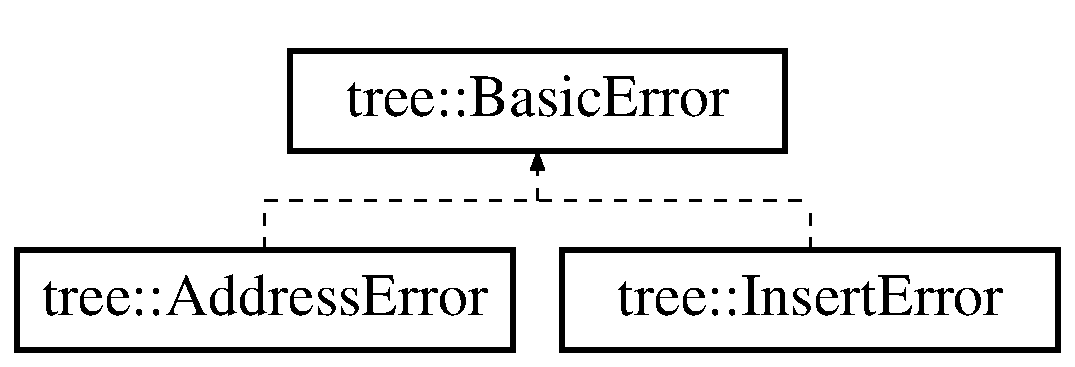
\includegraphics[height=2.000000cm]{classtree_1_1BasicError}
\end{center}
\end{figure}
\subsection*{Public Member Functions}
\begin{DoxyCompactItemize}
\item 
\hypertarget{classtree_1_1BasicError_ae973255633ffda1f9e05043683c3114e}{{\bfseries Basic\-Error} (const \hyperlink{classnode_1_1Node}{node\-::\-Node} $\ast$const i\-Pointer=N\-U\-L\-L)}\label{classtree_1_1BasicError_ae973255633ffda1f9e05043683c3114e}

\end{DoxyCompactItemize}
\subsection*{Protected Attributes}
\begin{DoxyCompactItemize}
\item 
\hypertarget{classtree_1_1BasicError_a5f85bebe161925ca7e059c4a905f7ac4}{const \hyperlink{classnode_1_1Node}{node\-::\-Node} $\ast$const {\bfseries e\-Pointer}}\label{classtree_1_1BasicError_a5f85bebe161925ca7e059c4a905f7ac4}

\end{DoxyCompactItemize}


\subsection{Detailed Description}
Basic error class. 

Definition at line 15 of file tree.\-hpp.



The documentation for this class was generated from the following file\-:\begin{DoxyCompactItemize}
\item 
src/tree.\-hpp\end{DoxyCompactItemize}

\hypertarget{classnode_1_1BasicError}{\section{node\-:\-:Basic\-Error Class Reference}
\label{classnode_1_1BasicError}\index{node\-::\-Basic\-Error@{node\-::\-Basic\-Error}}
}


Basic error class.  




{\ttfamily \#include $<$node.\-hpp$>$}

Inheritance diagram for node\-:\-:Basic\-Error\-:\begin{figure}[H]
\begin{center}
\leavevmode
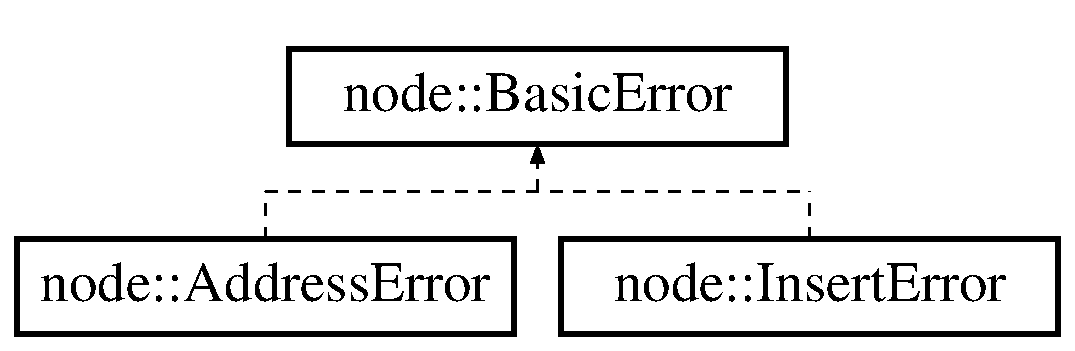
\includegraphics[height=2.000000cm]{classnode_1_1BasicError}
\end{center}
\end{figure}
\subsection*{Public Member Functions}
\begin{DoxyCompactItemize}
\item 
\hypertarget{classnode_1_1BasicError_a020ac995e67f64fdb4fcf3935f85fc8e}{{\bfseries Basic\-Error} (const \hyperlink{classnode_1_1Node}{Node} $\ast$const i\-Pointer=N\-U\-L\-L)}\label{classnode_1_1BasicError_a020ac995e67f64fdb4fcf3935f85fc8e}

\end{DoxyCompactItemize}
\subsection*{Protected Attributes}
\begin{DoxyCompactItemize}
\item 
\hypertarget{classnode_1_1BasicError_a8fb9d37c1e6c81e2c1f08c6ed10c4468}{const \hyperlink{classnode_1_1Node}{Node} $\ast$const {\bfseries e\-Pointer}}\label{classnode_1_1BasicError_a8fb9d37c1e6c81e2c1f08c6ed10c4468}

\end{DoxyCompactItemize}


\subsection{Detailed Description}
Basic error class. 

Definition at line 10 of file node.\-hpp.



The documentation for this class was generated from the following file\-:\begin{DoxyCompactItemize}
\item 
src/node.\-hpp\end{DoxyCompactItemize}

\hypertarget{classnode_1_1InsertError}{\section{node\-:\-:Insert\-Error Class Reference}
\label{classnode_1_1InsertError}\index{node\-::\-Insert\-Error@{node\-::\-Insert\-Error}}
}


Thrown if try to add node to busy place.  




{\ttfamily \#include $<$node.\-hpp$>$}

Inheritance diagram for node\-:\-:Insert\-Error\-:\begin{figure}[H]
\begin{center}
\leavevmode
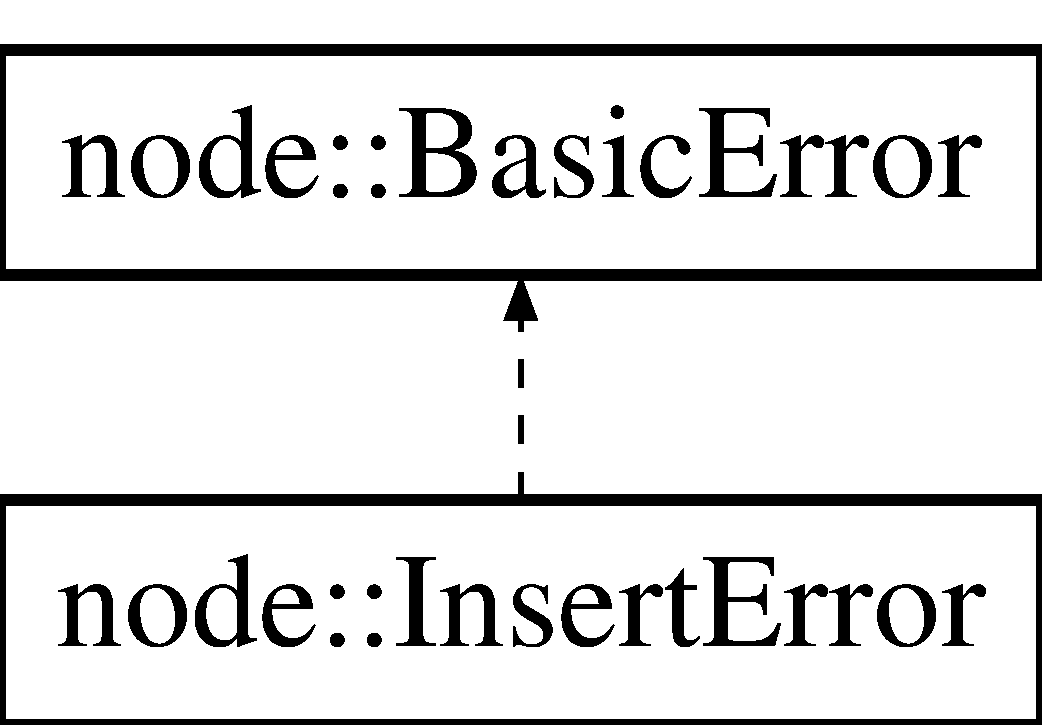
\includegraphics[height=2.000000cm]{classnode_1_1InsertError}
\end{center}
\end{figure}
\subsection*{Public Member Functions}
\begin{DoxyCompactItemize}
\item 
\hypertarget{classnode_1_1InsertError_a72063653683422110d5736d16a7bf54e}{{\bfseries Insert\-Error} (const \hyperlink{classnode_1_1Node}{Node} $\ast$const i\-Pointer=N\-U\-L\-L)}\label{classnode_1_1InsertError_a72063653683422110d5736d16a7bf54e}

\item 
\hypertarget{classnode_1_1InsertError_adfdbe66e711c6986d0ed0ebbfb06b90f}{std\-::ostream \& {\bfseries operator$<$$<$} (std\-::ostream \&os)}\label{classnode_1_1InsertError_adfdbe66e711c6986d0ed0ebbfb06b90f}

\end{DoxyCompactItemize}
\subsection*{Additional Inherited Members}


\subsection{Detailed Description}
Thrown if try to add node to busy place. 

Definition at line 19 of file node.\-hpp.



The documentation for this class was generated from the following file\-:\begin{DoxyCompactItemize}
\item 
src/node.\-hpp\end{DoxyCompactItemize}

\hypertarget{classtree_1_1InsertError}{\section{tree\-:\-:Insert\-Error Class Reference}
\label{classtree_1_1InsertError}\index{tree\-::\-Insert\-Error@{tree\-::\-Insert\-Error}}
}


Thrown if try to add something to busy place.  




{\ttfamily \#include $<$tree.\-hpp$>$}

Inheritance diagram for tree\-:\-:Insert\-Error\-:\begin{figure}[H]
\begin{center}
\leavevmode
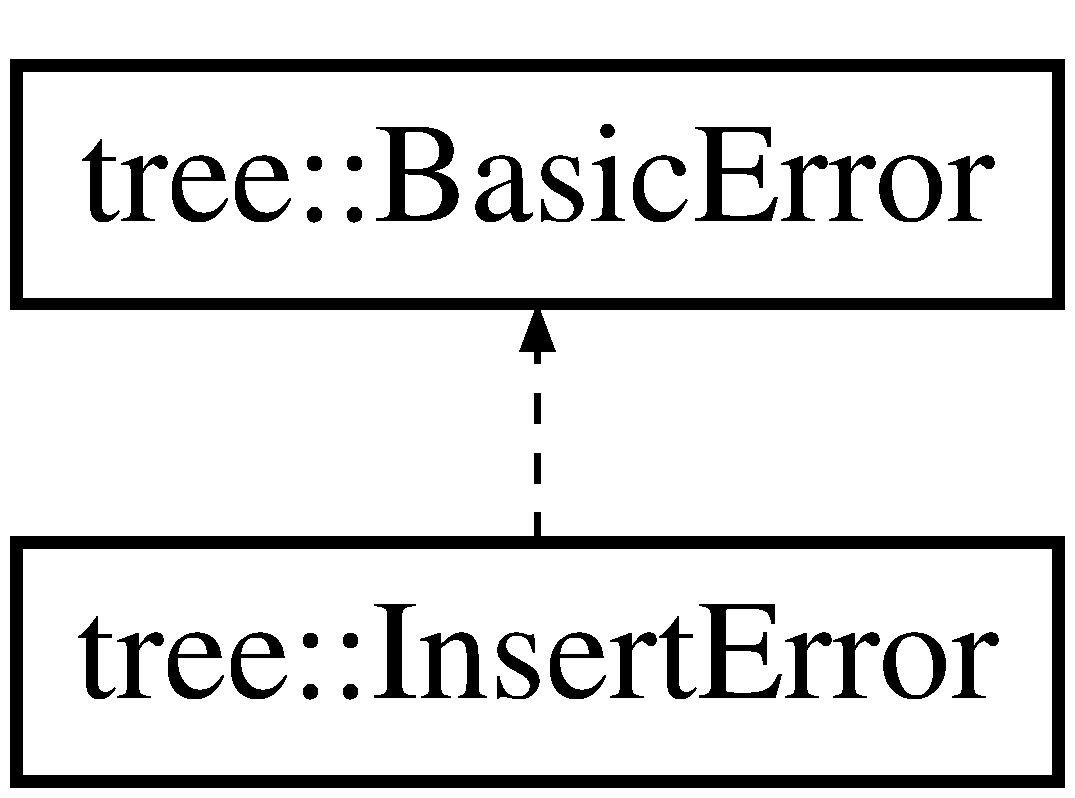
\includegraphics[height=2.000000cm]{classtree_1_1InsertError}
\end{center}
\end{figure}
\subsection*{Public Member Functions}
\begin{DoxyCompactItemize}
\item 
\hypertarget{classtree_1_1InsertError_a67b549c6063a756f96721c03ca51a6e3}{{\bfseries Insert\-Error} (const \hyperlink{classnode_1_1Node}{node\-::\-Node} $\ast$const i\-Pointer=N\-U\-L\-L)}\label{classtree_1_1InsertError_a67b549c6063a756f96721c03ca51a6e3}

\end{DoxyCompactItemize}
\subsection*{Friends}
\begin{DoxyCompactItemize}
\item 
\hypertarget{classtree_1_1InsertError_a85bf7765cbb99dba68bd7ca692ded69e}{std\-::ostream \& {\bfseries operator$<$$<$} (std\-::ostream \&os, const \hyperlink{classtree_1_1InsertError}{Insert\-Error} \&e)}\label{classtree_1_1InsertError_a85bf7765cbb99dba68bd7ca692ded69e}

\end{DoxyCompactItemize}
\subsection*{Additional Inherited Members}


\subsection{Detailed Description}
Thrown if try to add something to busy place. 

Definition at line 24 of file tree.\-hpp.



The documentation for this class was generated from the following file\-:\begin{DoxyCompactItemize}
\item 
src/tree.\-hpp\end{DoxyCompactItemize}

\hypertarget{classnode_1_1Node}{\section{node\-:\-:Node Class Reference}
\label{classnode_1_1Node}\index{node\-::\-Node@{node\-::\-Node}}
}


This class provides atomized operations relationed to current node.  




{\ttfamily \#include $<$node.\-hpp$>$}

\subsection*{Public Member Functions}
\begin{DoxyCompactItemize}
\item 
\hypertarget{classnode_1_1Node_a5caad933e458d07b106592c3adc57376}{\hyperlink{classnode_1_1Node_a5caad933e458d07b106592c3adc57376}{Node} ()}\label{classnode_1_1Node_a5caad933e458d07b106592c3adc57376}

\begin{DoxyCompactList}\small\item\em Creates node with empty name and zero level. \end{DoxyCompactList}\item 
\hyperlink{classnode_1_1Node_a8ed9e1fe9979ed9fefa4596a7d3f9098}{Node} (const std\-::string \&i\-Name)
\begin{DoxyCompactList}\small\item\em Creates node with specified name and zero level. \end{DoxyCompactList}\item 
\hyperlink{classnode_1_1Node_a214bbdde99347bda1d92a4b9ebee421c}{Node} (const \hyperlink{classnode_1_1Node}{Node} \&i\-Node)
\begin{DoxyCompactList}\small\item\em Copy constructor. \end{DoxyCompactList}\item 
\hypertarget{classnode_1_1Node_a4594558bd19fa4633a0ec277950c281f}{\hyperlink{classnode_1_1Node_a4594558bd19fa4633a0ec277950c281f}{$\sim$\-Node} ()}\label{classnode_1_1Node_a4594558bd19fa4633a0ec277950c281f}

\begin{DoxyCompactList}\small\item\em Recursive destructor. \end{DoxyCompactList}\item 
\hyperlink{classnode_1_1Node}{Node} \& \hyperlink{classnode_1_1Node_a77e2492642e7741f301ea12bc943ff79}{get\-Left} () const 
\begin{DoxyCompactList}\small\item\em Get reference to left child. \end{DoxyCompactList}\item 
\hyperlink{classnode_1_1Node}{Node} \& \hyperlink{classnode_1_1Node_a49ca4f8e2c62bfec66bec4ec4be0ce42}{get\-Right} () const 
\begin{DoxyCompactList}\small\item\em Get reference to right child. \end{DoxyCompactList}\item 
\hyperlink{classnode_1_1Node}{Node} \& \hyperlink{classnode_1_1Node_ad9daef61614061d0d2d7da0dfd425ff1}{get\-Top} () const 
\begin{DoxyCompactList}\small\item\em Get reference to parent node. \end{DoxyCompactList}\item 
\hyperlink{classnode_1_1Node}{Node} \& \hyperlink{classnode_1_1Node_ae31c4cd9619b2c968631bf58c915233f}{add\-Left} (const std\-::string \&i\-Name)
\begin{DoxyCompactList}\small\item\em Adds left child. \end{DoxyCompactList}\item 
\hyperlink{classnode_1_1Node}{Node} \& \hyperlink{classnode_1_1Node_a853bb602104e4e65d0d17e1a38dcfb94}{add\-Left} (const \hyperlink{classnode_1_1Node}{Node} \&i\-Node)
\begin{DoxyCompactList}\small\item\em Adds left child. \end{DoxyCompactList}\item 
\hyperlink{classnode_1_1Node}{Node} \& \hyperlink{classnode_1_1Node_a8a676071ac063cf27a13bcdd316a673b}{add\-Right} (const std\-::string \&i\-Name)
\begin{DoxyCompactList}\small\item\em Adds right child. \end{DoxyCompactList}\item 
\hyperlink{classnode_1_1Node}{Node} \& \hyperlink{classnode_1_1Node_a85be9468caa1a9f8e7976e5f30166b8d}{add\-Right} (const \hyperlink{classnode_1_1Node}{Node} \&i\-Node)
\begin{DoxyCompactList}\small\item\em Adds left child. \end{DoxyCompactList}\item 
\hypertarget{classnode_1_1Node_adaff3f88360e19f705fa729aea7adb43}{\hyperlink{classnode_1_1Node}{Node} \& \hyperlink{classnode_1_1Node_adaff3f88360e19f705fa729aea7adb43}{delete\-Left} ()}\label{classnode_1_1Node_adaff3f88360e19f705fa729aea7adb43}

\begin{DoxyCompactList}\small\item\em Deletes left subtree. \end{DoxyCompactList}\item 
\hypertarget{classnode_1_1Node_a00fc2ecb534c80527e8b42f4be3084a5}{\hyperlink{classnode_1_1Node}{Node} \& \hyperlink{classnode_1_1Node_a00fc2ecb534c80527e8b42f4be3084a5}{delete\-Right} ()}\label{classnode_1_1Node_a00fc2ecb534c80527e8b42f4be3084a5}

\begin{DoxyCompactList}\small\item\em Deletes right subtree. \end{DoxyCompactList}\item 
\hypertarget{classnode_1_1Node_abd035403eb1ce41e220f036595717d98}{std\-::string \hyperlink{classnode_1_1Node_abd035403eb1ce41e220f036595717d98}{get\-Name} () const }\label{classnode_1_1Node_abd035403eb1ce41e220f036595717d98}

\begin{DoxyCompactList}\small\item\em Get node name. \end{DoxyCompactList}\item 
\hypertarget{classnode_1_1Node_a6cec5b63d685d29a2d849336a8d6f8d2}{\hyperlink{classnode_1_1Node}{Node} \& \hyperlink{classnode_1_1Node_a6cec5b63d685d29a2d849336a8d6f8d2}{set\-Name} (const std\-::string \&i\-Name)}\label{classnode_1_1Node_a6cec5b63d685d29a2d849336a8d6f8d2}

\begin{DoxyCompactList}\small\item\em Set node name. \end{DoxyCompactList}\item 
\hyperlink{classnode_1_1Node}{Node} \& \hyperlink{classnode_1_1Node_af6e99944cbf63f15cd85ecb4655bde6e}{operator=} (const \hyperlink{classnode_1_1Node}{Node} \&i\-Node)
\begin{DoxyCompactList}\small\item\em Sets current node equal to {\itshape copy} of specified node structure. \end{DoxyCompactList}\item 
\hyperlink{classnode_1_1Node}{Node} \& \hyperlink{classnode_1_1Node_a75716ea94259082ba459234bdf45be50}{operator=} (const std\-::string \&i\-Name)
\begin{DoxyCompactList}\small\item\em Sets current node equal to node with specified name. \end{DoxyCompactList}\item 
\hyperlink{classnode_1_1Node}{Node} \& \hyperlink{classnode_1_1Node_aedae3083215e9f9785d3d9d655a26fc7}{operator$<$} (const \hyperlink{classnode_1_1Node}{Node} \&i\-Node)
\begin{DoxyCompactList}\small\item\em Adds specified node structure as left child. \end{DoxyCompactList}\item 
\hyperlink{classnode_1_1Node}{Node} \& \hyperlink{classnode_1_1Node_ad9bf2bb992fb6c363fb2cdf6d5fd7924}{operator$<$} (const std\-::string \&i\-Name)
\begin{DoxyCompactList}\small\item\em Adds node with specified name as left child. \end{DoxyCompactList}\item 
\hyperlink{classnode_1_1Node}{Node} \& \hyperlink{classnode_1_1Node_a74195c5033e17798b6ad909765012317}{operator$>$} (const \hyperlink{classnode_1_1Node}{Node} \&i\-Node)
\begin{DoxyCompactList}\small\item\em Adds specified node structure as right child. Normalizes inserted subtree. Throws \hyperlink{classnode_1_1InsertError}{node\-::\-Insert\-Error} exception if try to insert i\-Node to busy place. \end{DoxyCompactList}\item 
\hyperlink{classnode_1_1Node}{Node} \& \hyperlink{classnode_1_1Node_a92db84e7ddf68b555800f72621745311}{operator$>$} (const std\-::string \&i\-Name)
\begin{DoxyCompactList}\small\item\em Adds node with specified name as right child. Throws \hyperlink{classnode_1_1InsertError}{node\-::\-Insert\-Error} exception if try to insert i\-Node to busy place. \end{DoxyCompactList}\item 
\hypertarget{classnode_1_1Node_a1d1940dc3b8285207c7746bcf9569926}{unsigned int \hyperlink{classnode_1_1Node_a1d1940dc3b8285207c7746bcf9569926}{get\-Level} () const }\label{classnode_1_1Node_a1d1940dc3b8285207c7746bcf9569926}

\begin{DoxyCompactList}\small\item\em Get node level. \end{DoxyCompactList}\item 
\hypertarget{classnode_1_1Node_a7b5de538f317d34fbcd050ee22e1d6af}{unsigned int \hyperlink{classnode_1_1Node_a7b5de538f317d34fbcd050ee22e1d6af}{normalize\-Level} ()}\label{classnode_1_1Node_a7b5de538f317d34fbcd050ee22e1d6af}

\begin{DoxyCompactList}\small\item\em Makes node levels growing in order, counted form root. Root level == 0. Returns counted depth of tree. \end{DoxyCompactList}\end{DoxyCompactItemize}
\subsection*{Friends}
\begin{DoxyCompactItemize}
\item 
void \hyperlink{classnode_1_1Node_a64879d4c1aca07f9dd96e28e5bf988a4}{\-\_\-connect} (\hyperlink{classnode_1_1Node}{Node} $\ast$c\-Node, const \hyperlink{classnode_1_1Node}{Node} $\ast$p\-Node)
\begin{DoxyCompactList}\small\item\em Set pointer to parent of current node to selected node. \end{DoxyCompactList}\end{DoxyCompactItemize}


\subsection{Detailed Description}
This class provides atomized operations relationed to current node. 

Definition at line 51 of file node.\-hpp.



\subsection{Constructor \& Destructor Documentation}
\hypertarget{classnode_1_1Node_a8ed9e1fe9979ed9fefa4596a7d3f9098}{\index{node\-::\-Node@{node\-::\-Node}!Node@{Node}}
\index{Node@{Node}!node::Node@{node\-::\-Node}}
\subsubsection[{Node}]{\setlength{\rightskip}{0pt plus 5cm}node\-::\-Node\-::\-Node (
\begin{DoxyParamCaption}
\item[{const std\-::string \&}]{i\-Name}
\end{DoxyParamCaption}
)}}\label{classnode_1_1Node_a8ed9e1fe9979ed9fefa4596a7d3f9098}


Creates node with specified name and zero level. 


\begin{DoxyParams}{Parameters}
{\em i\-Name} & -- name for node. \\
\hline
\end{DoxyParams}


Definition at line 109 of file node.\-hpp.

\hypertarget{classnode_1_1Node_a214bbdde99347bda1d92a4b9ebee421c}{\index{node\-::\-Node@{node\-::\-Node}!Node@{Node}}
\index{Node@{Node}!node::Node@{node\-::\-Node}}
\subsubsection[{Node}]{\setlength{\rightskip}{0pt plus 5cm}node\-::\-Node\-::\-Node (
\begin{DoxyParamCaption}
\item[{const {\bf Node} \&}]{i\-Node}
\end{DoxyParamCaption}
)}}\label{classnode_1_1Node_a214bbdde99347bda1d92a4b9ebee421c}


Copy constructor. 

Creates node from other node structure. Level may be not normalized, but grown. 
\begin{DoxyParams}{Parameters}
{\em i\-Node} & -- source node to copy. \\
\hline
\end{DoxyParams}


Definition at line 122 of file node.\-hpp.



\subsection{Member Function Documentation}
\hypertarget{classnode_1_1Node_ae31c4cd9619b2c968631bf58c915233f}{\index{node\-::\-Node@{node\-::\-Node}!add\-Left@{add\-Left}}
\index{add\-Left@{add\-Left}!node::Node@{node\-::\-Node}}
\subsubsection[{add\-Left}]{\setlength{\rightskip}{0pt plus 5cm}{\bf Node} \& node\-::\-Node\-::add\-Left (
\begin{DoxyParamCaption}
\item[{const std\-::string \&}]{i\-Name}
\end{DoxyParamCaption}
)}}\label{classnode_1_1Node_ae31c4cd9619b2c968631bf58c915233f}


Adds left child. 

Inserts node with specified name as left child, if not exists. Normalizes inserted node. Throws \hyperlink{classnode_1_1InsertError}{node\-::\-Insert\-Error} exception in other way.


\begin{DoxyParams}{Parameters}
{\em i\-Name} & -- name of node to insert. \\
\hline
\end{DoxyParams}


Definition at line 215 of file node.\-hpp.

\hypertarget{classnode_1_1Node_a853bb602104e4e65d0d17e1a38dcfb94}{\index{node\-::\-Node@{node\-::\-Node}!add\-Left@{add\-Left}}
\index{add\-Left@{add\-Left}!node::Node@{node\-::\-Node}}
\subsubsection[{add\-Left}]{\setlength{\rightskip}{0pt plus 5cm}{\bf Node} \& node\-::\-Node\-::add\-Left (
\begin{DoxyParamCaption}
\item[{const {\bf Node} \&}]{i\-Node}
\end{DoxyParamCaption}
)}}\label{classnode_1_1Node_a853bb602104e4e65d0d17e1a38dcfb94}


Adds left child. 

Inserts node structure as left child, if not exists. Normalizes inserted subtree. Throws \hyperlink{classnode_1_1InsertError}{node\-::\-Insert\-Error} exception in other way.


\begin{DoxyParams}{Parameters}
{\em i\-Node} & -- source of node structure to insert. \\
\hline
\end{DoxyParams}


Definition at line 237 of file node.\-hpp.

\hypertarget{classnode_1_1Node_a8a676071ac063cf27a13bcdd316a673b}{\index{node\-::\-Node@{node\-::\-Node}!add\-Right@{add\-Right}}
\index{add\-Right@{add\-Right}!node::Node@{node\-::\-Node}}
\subsubsection[{add\-Right}]{\setlength{\rightskip}{0pt plus 5cm}{\bf Node} \& node\-::\-Node\-::add\-Right (
\begin{DoxyParamCaption}
\item[{const std\-::string \&}]{i\-Name}
\end{DoxyParamCaption}
)}}\label{classnode_1_1Node_a8a676071ac063cf27a13bcdd316a673b}


Adds right child. 

Inserts node with specified name as right child, if not exists. Normalizes inserted node. Throws \hyperlink{classnode_1_1InsertError}{node\-::\-Insert\-Error} exception in other way.


\begin{DoxyParams}{Parameters}
{\em i\-Name} & -- name of node to insert. \\
\hline
\end{DoxyParams}


Definition at line 258 of file node.\-hpp.

\hypertarget{classnode_1_1Node_a85be9468caa1a9f8e7976e5f30166b8d}{\index{node\-::\-Node@{node\-::\-Node}!add\-Right@{add\-Right}}
\index{add\-Right@{add\-Right}!node::Node@{node\-::\-Node}}
\subsubsection[{add\-Right}]{\setlength{\rightskip}{0pt plus 5cm}{\bf Node} \& node\-::\-Node\-::add\-Right (
\begin{DoxyParamCaption}
\item[{const {\bf Node} \&}]{i\-Node}
\end{DoxyParamCaption}
)}}\label{classnode_1_1Node_a85be9468caa1a9f8e7976e5f30166b8d}


Adds left child. 

Inserts node structure as right child, if not exists. Normalizes inserted subtree. Throws \hyperlink{classnode_1_1InsertError}{node\-::\-Insert\-Error} exception in other way.


\begin{DoxyParams}{Parameters}
{\em i\-Node} & -- source of node structure to insert. \\
\hline
\end{DoxyParams}


Definition at line 280 of file node.\-hpp.

\hypertarget{classnode_1_1Node_a77e2492642e7741f301ea12bc943ff79}{\index{node\-::\-Node@{node\-::\-Node}!get\-Left@{get\-Left}}
\index{get\-Left@{get\-Left}!node::Node@{node\-::\-Node}}
\subsubsection[{get\-Left}]{\setlength{\rightskip}{0pt plus 5cm}{\bf Node} \& node\-::\-Node\-::get\-Left (
\begin{DoxyParamCaption}
{}
\end{DoxyParamCaption}
) const}}\label{classnode_1_1Node_a77e2492642e7741f301ea12bc943ff79}


Get reference to left child. 

Returns reference to left child, if exists. Throws \hyperlink{classnode_1_1AddressError}{node\-::\-Address\-Error} exception in other way. 

Definition at line 175 of file node.\-hpp.

\hypertarget{classnode_1_1Node_a49ca4f8e2c62bfec66bec4ec4be0ce42}{\index{node\-::\-Node@{node\-::\-Node}!get\-Right@{get\-Right}}
\index{get\-Right@{get\-Right}!node::Node@{node\-::\-Node}}
\subsubsection[{get\-Right}]{\setlength{\rightskip}{0pt plus 5cm}{\bf Node} \& node\-::\-Node\-::get\-Right (
\begin{DoxyParamCaption}
{}
\end{DoxyParamCaption}
) const}}\label{classnode_1_1Node_a49ca4f8e2c62bfec66bec4ec4be0ce42}


Get reference to right child. 

Returns reference to right child, if exists. Throws \hyperlink{classnode_1_1AddressError}{node\-::\-Address\-Error} exception in other way. 

Definition at line 187 of file node.\-hpp.

\hypertarget{classnode_1_1Node_ad9daef61614061d0d2d7da0dfd425ff1}{\index{node\-::\-Node@{node\-::\-Node}!get\-Top@{get\-Top}}
\index{get\-Top@{get\-Top}!node::Node@{node\-::\-Node}}
\subsubsection[{get\-Top}]{\setlength{\rightskip}{0pt plus 5cm}{\bf Node} \& node\-::\-Node\-::get\-Top (
\begin{DoxyParamCaption}
{}
\end{DoxyParamCaption}
) const}}\label{classnode_1_1Node_ad9daef61614061d0d2d7da0dfd425ff1}


Get reference to parent node. 

Returns reference to parent node, if exists. Throws \hyperlink{classnode_1_1AddressError}{node\-::\-Address\-Error} exception in other way. 

Definition at line 200 of file node.\-hpp.

\hypertarget{classnode_1_1Node_aedae3083215e9f9785d3d9d655a26fc7}{\index{node\-::\-Node@{node\-::\-Node}!operator$<$@{operator$<$}}
\index{operator$<$@{operator$<$}!node::Node@{node\-::\-Node}}
\subsubsection[{operator$<$}]{\setlength{\rightskip}{0pt plus 5cm}{\bf Node} \& node\-::\-Node\-::operator$<$ (
\begin{DoxyParamCaption}
\item[{const {\bf Node} \&}]{i\-Node}
\end{DoxyParamCaption}
)}}\label{classnode_1_1Node_aedae3083215e9f9785d3d9d655a26fc7}


Adds specified node structure as left child. 

Normalizes inserted subtree. Throws \hyperlink{classnode_1_1InsertError}{node\-::\-Insert\-Error} exception if try to insert i\-Node to busy place.


\begin{DoxyParams}{Parameters}
{\em i\-Node} & -- source node structure inserted node. \\
\hline
\end{DoxyParams}


Definition at line 351 of file node.\-hpp.

\hypertarget{classnode_1_1Node_ad9bf2bb992fb6c363fb2cdf6d5fd7924}{\index{node\-::\-Node@{node\-::\-Node}!operator$<$@{operator$<$}}
\index{operator$<$@{operator$<$}!node::Node@{node\-::\-Node}}
\subsubsection[{operator$<$}]{\setlength{\rightskip}{0pt plus 5cm}{\bf Node} \& node\-::\-Node\-::operator$<$ (
\begin{DoxyParamCaption}
\item[{const std\-::string \&}]{i\-Name}
\end{DoxyParamCaption}
)}}\label{classnode_1_1Node_ad9bf2bb992fb6c363fb2cdf6d5fd7924}


Adds node with specified name as left child. 

Throws \hyperlink{classnode_1_1InsertError}{node\-::\-Insert\-Error} exception if try to insert i\-Node to busy place. Normalizes inserted node.


\begin{DoxyParams}{Parameters}
{\em i\-Name} & -- source name for node to insert. \\
\hline
\end{DoxyParams}


Definition at line 364 of file node.\-hpp.

\hypertarget{classnode_1_1Node_af6e99944cbf63f15cd85ecb4655bde6e}{\index{node\-::\-Node@{node\-::\-Node}!operator=@{operator=}}
\index{operator=@{operator=}!node::Node@{node\-::\-Node}}
\subsubsection[{operator=}]{\setlength{\rightskip}{0pt plus 5cm}{\bf Node} \& node\-::\-Node\-::operator= (
\begin{DoxyParamCaption}
\item[{const {\bf Node} \&}]{i\-Node}
\end{DoxyParamCaption}
)}}\label{classnode_1_1Node_af6e99944cbf63f15cd85ecb4655bde6e}


Sets current node equal to {\itshape copy} of specified node structure. 


\begin{DoxyParams}{Parameters}
{\em i\-Node} & -- source node structure. \\
\hline
\end{DoxyParams}


Definition at line 314 of file node.\-hpp.

\hypertarget{classnode_1_1Node_a75716ea94259082ba459234bdf45be50}{\index{node\-::\-Node@{node\-::\-Node}!operator=@{operator=}}
\index{operator=@{operator=}!node::Node@{node\-::\-Node}}
\subsubsection[{operator=}]{\setlength{\rightskip}{0pt plus 5cm}{\bf Node} \& node\-::\-Node\-::operator= (
\begin{DoxyParamCaption}
\item[{const std\-::string \&}]{i\-Name}
\end{DoxyParamCaption}
)}}\label{classnode_1_1Node_a75716ea94259082ba459234bdf45be50}


Sets current node equal to node with specified name. 


\begin{DoxyParams}{Parameters}
{\em i\-Name} & -- source name for node to replace. \\
\hline
\end{DoxyParams}


Definition at line 336 of file node.\-hpp.

\hypertarget{classnode_1_1Node_a74195c5033e17798b6ad909765012317}{\index{node\-::\-Node@{node\-::\-Node}!operator$>$@{operator$>$}}
\index{operator$>$@{operator$>$}!node::Node@{node\-::\-Node}}
\subsubsection[{operator$>$}]{\setlength{\rightskip}{0pt plus 5cm}{\bf Node} \& node\-::\-Node\-::operator$>$ (
\begin{DoxyParamCaption}
\item[{const {\bf Node} \&}]{i\-Node}
\end{DoxyParamCaption}
)}}\label{classnode_1_1Node_a74195c5033e17798b6ad909765012317}


Adds specified node structure as right child. Normalizes inserted subtree. Throws \hyperlink{classnode_1_1InsertError}{node\-::\-Insert\-Error} exception if try to insert i\-Node to busy place. 


\begin{DoxyParams}{Parameters}
{\em i\-Node} & -- source node structure inserted node. \\
\hline
\end{DoxyParams}


Definition at line 376 of file node.\-hpp.

\hypertarget{classnode_1_1Node_a92db84e7ddf68b555800f72621745311}{\index{node\-::\-Node@{node\-::\-Node}!operator$>$@{operator$>$}}
\index{operator$>$@{operator$>$}!node::Node@{node\-::\-Node}}
\subsubsection[{operator$>$}]{\setlength{\rightskip}{0pt plus 5cm}{\bf Node} \& node\-::\-Node\-::operator$>$ (
\begin{DoxyParamCaption}
\item[{const std\-::string \&}]{i\-Name}
\end{DoxyParamCaption}
)}}\label{classnode_1_1Node_a92db84e7ddf68b555800f72621745311}


Adds node with specified name as right child. Throws \hyperlink{classnode_1_1InsertError}{node\-::\-Insert\-Error} exception if try to insert i\-Node to busy place. 


\begin{DoxyParams}{Parameters}
{\em i\-Name} & -- source name for node to insert. \\
\hline
\end{DoxyParams}


Definition at line 387 of file node.\-hpp.



\subsection{Friends And Related Function Documentation}
\hypertarget{classnode_1_1Node_a64879d4c1aca07f9dd96e28e5bf988a4}{\index{node\-::\-Node@{node\-::\-Node}!\-\_\-connect@{\-\_\-connect}}
\index{\-\_\-connect@{\-\_\-connect}!node::Node@{node\-::\-Node}}
\subsubsection[{\-\_\-connect}]{\setlength{\rightskip}{0pt plus 5cm}void \-\_\-connect (
\begin{DoxyParamCaption}
\item[{{\bf Node} $\ast$}]{c\-Node, }
\item[{const {\bf Node} $\ast$}]{p\-Node}
\end{DoxyParamCaption}
)\hspace{0.3cm}{\ttfamily [friend]}}}\label{classnode_1_1Node_a64879d4c1aca07f9dd96e28e5bf988a4}


Set pointer to parent of current node to selected node. 


\begin{DoxyParams}{Parameters}
{\em c\-Node} & -- current \hyperlink{classnode_1_1Node}{Node} \\
\hline
{\em p\-Node} & -- parent \hyperlink{classnode_1_1Node}{Node} \\
\hline
\end{DoxyParams}


Definition at line 415 of file node.\-hpp.



The documentation for this class was generated from the following file\-:\begin{DoxyCompactItemize}
\item 
src/node.\-hpp\end{DoxyCompactItemize}

\hypertarget{classtree_1_1Tree}{\section{tree\-:\-:Tree Class Reference}
\label{classtree_1_1Tree}\index{tree\-::\-Tree@{tree\-::\-Tree}}
}


Used for encapsulate \hyperlink{classnode_1_1Node}{node\-::\-Node} structures.  




{\ttfamily \#include $<$tree.\-hpp$>$}

\subsection*{Public Member Functions}
\begin{DoxyCompactItemize}
\item 
\hypertarget{classtree_1_1Tree_a66755a8dbcf714aa93e63952bdb62484}{\hyperlink{classtree_1_1Tree_a66755a8dbcf714aa93e63952bdb62484}{Tree} ()}\label{classtree_1_1Tree_a66755a8dbcf714aa93e63952bdb62484}

\begin{DoxyCompactList}\small\item\em Creates tree with unnamed node and depth == 1. \end{DoxyCompactList}\item 
\hyperlink{classtree_1_1Tree_ac9e85c2936a0c63f4928ac9864e487fb}{Tree} (const std\-::string \&i\-Name)
\begin{DoxyCompactList}\small\item\em Creates tree with specified name and depth == 1. \end{DoxyCompactList}\item 
\hyperlink{classtree_1_1Tree_ad55803fa67e5cd1f1f8b7b80e014ffaa}{Tree} (const \hyperlink{classnode_1_1Node}{node\-::\-Node} \&i\-Node)
\begin{DoxyCompactList}\small\item\em Creates tree from \hyperlink{classnode_1_1Node}{node\-::\-Node} structure. \end{DoxyCompactList}\item 
\hyperlink{classtree_1_1Tree_a71b78c230e92b439dfaab0fe4c9c956c}{Tree} (const \hyperlink{classtree_1_1Tree}{tree\-::\-Tree} \&i\-Tree)
\begin{DoxyCompactList}\small\item\em Creates tree from other tree. \end{DoxyCompactList}\item 
\hyperlink{classtree_1_1Tree}{Tree} \& \hyperlink{classtree_1_1Tree_a73dc8a4574c7222c6640c88eef387a19}{add\-Left} (const std\-::string \&i\-Name)
\begin{DoxyCompactList}\small\item\em Adds left child. \end{DoxyCompactList}\item 
\hyperlink{classtree_1_1Tree}{Tree} \& \hyperlink{classtree_1_1Tree_a6d98f5bb78258d03882041c6d6438ab0}{add\-Left} (const \hyperlink{classnode_1_1Node}{node\-::\-Node} \&i\-Node)
\begin{DoxyCompactList}\small\item\em Adds left child. \end{DoxyCompactList}\item 
\hyperlink{classtree_1_1Tree}{Tree} \& \hyperlink{classtree_1_1Tree_a73996a043448192cd9bb52175cd78a0c}{add\-Left} (const \hyperlink{classtree_1_1Tree}{Tree} \&i\-Tree)
\begin{DoxyCompactList}\small\item\em Adds left child. \end{DoxyCompactList}\item 
\hyperlink{classtree_1_1Tree}{Tree} \& \hyperlink{classtree_1_1Tree_a23e77e37d23040fabb35eeec86370b02}{add\-Right} (const std\-::string \&i\-Name)
\begin{DoxyCompactList}\small\item\em Adds right child. \end{DoxyCompactList}\item 
\hyperlink{classtree_1_1Tree}{Tree} \& \hyperlink{classtree_1_1Tree_aa4ac522514b647e10a087ea388868e31}{add\-Right} (const \hyperlink{classnode_1_1Node}{node\-::\-Node} \&i\-Node)
\begin{DoxyCompactList}\small\item\em Adds right child. \end{DoxyCompactList}\item 
\hyperlink{classtree_1_1Tree}{Tree} \& \hyperlink{classtree_1_1Tree_a1fe1a6b148f1ea7258e649f73e3b6a6f}{add\-Right} (const \hyperlink{classtree_1_1Tree}{Tree} \&i\-Tree)
\begin{DoxyCompactList}\small\item\em Adds right child. \end{DoxyCompactList}\item 
\hyperlink{classtree_1_1Tree}{Tree} \& \hyperlink{classtree_1_1Tree_af3de9693422e9af3e5b47f8bc386d821}{move\-Left} ()
\begin{DoxyCompactList}\small\item\em Move operation pointer to left child. \end{DoxyCompactList}\item 
\hyperlink{classtree_1_1Tree}{Tree} \& \hyperlink{classtree_1_1Tree_a783680aa05d80764a53353ab7b0ef1fb}{move\-Right} ()
\begin{DoxyCompactList}\small\item\em Move operation pointer to right child. \end{DoxyCompactList}\item 
\hypertarget{classtree_1_1Tree_ae664afeb1d788e51ceeb37d6720d7578}{\hyperlink{classtree_1_1Tree}{Tree} \& \hyperlink{classtree_1_1Tree_ae664afeb1d788e51ceeb37d6720d7578}{move\-Top} ()}\label{classtree_1_1Tree_ae664afeb1d788e51ceeb37d6720d7578}

\begin{DoxyCompactList}\small\item\em Move operation pointer to parent node. \end{DoxyCompactList}\item 
\hypertarget{classtree_1_1Tree_ad64be9c6cdaf79bfbc16b7e25ec7f072}{\hyperlink{classtree_1_1Tree}{Tree} \& \hyperlink{classtree_1_1Tree_ad64be9c6cdaf79bfbc16b7e25ec7f072}{move\-Root} ()}\label{classtree_1_1Tree_ad64be9c6cdaf79bfbc16b7e25ec7f072}

\begin{DoxyCompactList}\small\item\em Move operation pointer to root node. \end{DoxyCompactList}\item 
\hypertarget{classtree_1_1Tree_a1a3832a39a4b353766baf84316c692dc}{\hyperlink{classtree_1_1Tree}{Tree} \& \hyperlink{classtree_1_1Tree_a1a3832a39a4b353766baf84316c692dc}{delete\-Left} ()}\label{classtree_1_1Tree_a1a3832a39a4b353766baf84316c692dc}

\begin{DoxyCompactList}\small\item\em Deletes selected left subtree. \end{DoxyCompactList}\item 
\hypertarget{classtree_1_1Tree_af4ddc57ec2ed9629cd48dd34a2ab0645}{\hyperlink{classtree_1_1Tree}{Tree} \& \hyperlink{classtree_1_1Tree_af4ddc57ec2ed9629cd48dd34a2ab0645}{delete\-Right} ()}\label{classtree_1_1Tree_af4ddc57ec2ed9629cd48dd34a2ab0645}

\begin{DoxyCompactList}\small\item\em Deletes selected right subtree. \end{DoxyCompactList}\item 
\hypertarget{classtree_1_1Tree_afc485303d43f5ac66b074a9fc5d7d212}{std\-::string \hyperlink{classtree_1_1Tree_afc485303d43f5ac66b074a9fc5d7d212}{get\-Name} () const }\label{classtree_1_1Tree_afc485303d43f5ac66b074a9fc5d7d212}

\begin{DoxyCompactList}\small\item\em Get selected node name. \end{DoxyCompactList}\item 
\hypertarget{classtree_1_1Tree_aadbae7ca0bd170156b91d9f13d0fa783}{\hyperlink{classtree_1_1Tree}{Tree} \& \hyperlink{classtree_1_1Tree_aadbae7ca0bd170156b91d9f13d0fa783}{set\-Name} (const std\-::string \&i\-Name)}\label{classtree_1_1Tree_aadbae7ca0bd170156b91d9f13d0fa783}

\begin{DoxyCompactList}\small\item\em Set selected node name. \end{DoxyCompactList}\item 
\hyperlink{classtree_1_1Tree}{Tree} \& \hyperlink{classtree_1_1Tree_a87196f2bf4aac12cefe77df4515d1665}{operator=} (const \hyperlink{classtree_1_1Tree}{tree\-::\-Tree} \&i\-Tree)
\begin{DoxyCompactList}\small\item\em Sets content under operation pointer equal to {\itshape copy} of whole tree structure. \end{DoxyCompactList}\item 
\hyperlink{classtree_1_1Tree}{Tree} \& \hyperlink{classtree_1_1Tree_ab421f2c2b6ceab773cb5854317186791}{operator=} (const \hyperlink{classnode_1_1Node}{node\-::\-Node} \&i\-Node)
\begin{DoxyCompactList}\small\item\em Sets content under operation pointer equal to {\itshape copy} of specified node structure. \end{DoxyCompactList}\item 
\hyperlink{classtree_1_1Tree}{Tree} \& \hyperlink{classtree_1_1Tree_a310a51f2fecc6f93d57091c364fa4d99}{operator=} (const std\-::string \&i\-Name)
\begin{DoxyCompactList}\small\item\em Sets content under operation pointer equal to node with specified name. \end{DoxyCompactList}\item 
\hyperlink{classtree_1_1Tree}{Tree} \& \hyperlink{classtree_1_1Tree_a3d8e27ab655fed7f4d7b640f30628312}{operator$<$} (const \hyperlink{classtree_1_1Tree}{tree\-::\-Tree} \&i\-Tree)
\begin{DoxyCompactList}\small\item\em Adds {\itshape copy} of whole source tree as left child of operation pointer. \end{DoxyCompactList}\item 
\hyperlink{classtree_1_1Tree}{Tree} \& \hyperlink{classtree_1_1Tree_afccc4be4d4097a231c48385a4c7fc402}{operator$<$} (const \hyperlink{classnode_1_1Node}{node\-::\-Node} \&i\-Node)
\begin{DoxyCompactList}\small\item\em Adds specified node structure as left child of operation pointer. \end{DoxyCompactList}\item 
\hyperlink{classtree_1_1Tree}{Tree} \& \hyperlink{classtree_1_1Tree_a9197395651b7b6098ffd2eeb62c39263}{operator$<$} (const std\-::string \&i\-Name)
\begin{DoxyCompactList}\small\item\em Adds node with specified name as left child of operation pointer. \end{DoxyCompactList}\item 
\hyperlink{classtree_1_1Tree}{Tree} \& \hyperlink{classtree_1_1Tree_aaffe009efda5ae4b6699890e9c1a7c30}{operator$>$} (const \hyperlink{classtree_1_1Tree}{tree\-::\-Tree} \&i\-Tree)
\begin{DoxyCompactList}\small\item\em Adds {\itshape copy} of whole source tree as right child of operation pointer. \end{DoxyCompactList}\item 
\hyperlink{classtree_1_1Tree}{Tree} \& \hyperlink{classtree_1_1Tree_ae058874c4bd591e2cb060806d6e9de41}{operator$>$} (const \hyperlink{classnode_1_1Node}{node\-::\-Node} \&i\-Node)
\begin{DoxyCompactList}\small\item\em Adds specified node structure as right child of operation pointer. \end{DoxyCompactList}\item 
\hyperlink{classtree_1_1Tree}{Tree} \& \hyperlink{classtree_1_1Tree_a438deea3b585e9f003d21c342e8ad4b1}{operator$>$} (const std\-::string \&i\-Name)
\begin{DoxyCompactList}\small\item\em Adds node with specified name as right child of operation pointer. \end{DoxyCompactList}\item 
\hypertarget{classtree_1_1Tree_a4ddf2644182f9fb72aea10cd42e27926}{unsigned int \hyperlink{classtree_1_1Tree_a4ddf2644182f9fb72aea10cd42e27926}{get\-Level} () const }\label{classtree_1_1Tree_a4ddf2644182f9fb72aea10cd42e27926}

\begin{DoxyCompactList}\small\item\em Get level of selected node. \end{DoxyCompactList}\item 
\hypertarget{classtree_1_1Tree_a88fbf6974cbb144273fffb8289599978}{unsigned int \hyperlink{classtree_1_1Tree_a88fbf6974cbb144273fffb8289599978}{get\-Depth} () const }\label{classtree_1_1Tree_a88fbf6974cbb144273fffb8289599978}

\begin{DoxyCompactList}\small\item\em Get tree depth. \end{DoxyCompactList}\item 
\hypertarget{classtree_1_1Tree_a8510242d20d1a62e694bdda7d6f08355}{\hyperlink{classnode_1_1Node}{node\-::\-Node} \& \hyperlink{classtree_1_1Tree_a8510242d20d1a62e694bdda7d6f08355}{get\-Nodes} () const }\label{classtree_1_1Tree_a8510242d20d1a62e694bdda7d6f08355}

\begin{DoxyCompactList}\small\item\em Get {\itshape copy} node structure of tree. \end{DoxyCompactList}\item 
\hyperlink{namespacetree_a36da3b38ad98fe87c16c4336cd5b8a44}{Tree\-Nodes} \hyperlink{classtree_1_1Tree_a4dce9d5202dc7412ec8f1432040d5deb}{search} (const std\-::string \&s\-Name) const 
\begin{DoxyCompactList}\small\item\em Finds nodes with specified name. \end{DoxyCompactList}\item 
\hypertarget{classtree_1_1Tree_ae84318b936a74cfd6f8ba2705b1bd6ac}{\hyperlink{namespacetree_a1906ab31086935949f162ea3e2c41200}{Tree\-Content} \hyperlink{classtree_1_1Tree_ae84318b936a74cfd6f8ba2705b1bd6ac}{get\-Content} () const }\label{classtree_1_1Tree_ae84318b936a74cfd6f8ba2705b1bd6ac}

\begin{DoxyCompactList}\small\item\em Gets tree content in vector-\/based representation. \end{DoxyCompactList}\item 
\hyperlink{namespacetree_a36da3b38ad98fe87c16c4336cd5b8a44}{Tree\-Nodes} \hyperlink{classtree_1_1Tree_a5ae3316bf8d3905413cc5454e5079b3f}{operator\mbox{[}$\,$\mbox{]}} (const std\-::string \&s\-Name) const 
\begin{DoxyCompactList}\small\item\em Finds nodes with specified name. \end{DoxyCompactList}\end{DoxyCompactItemize}


\subsection{Detailed Description}
Used for encapsulate \hyperlink{classnode_1_1Node}{node\-::\-Node} structures. 

This class provides tree-\/oriented operations based on \hyperlink{classnode_1_1Node}{node\-::\-Node} class. 

Definition at line 50 of file tree.\-hpp.



\subsection{Constructor \& Destructor Documentation}
\hypertarget{classtree_1_1Tree_ac9e85c2936a0c63f4928ac9864e487fb}{\index{tree\-::\-Tree@{tree\-::\-Tree}!Tree@{Tree}}
\index{Tree@{Tree}!tree::Tree@{tree\-::\-Tree}}
\subsubsection[{Tree}]{\setlength{\rightskip}{0pt plus 5cm}tree\-::\-Tree\-::\-Tree (
\begin{DoxyParamCaption}
\item[{const std\-::string \&}]{i\-Name}
\end{DoxyParamCaption}
)\hspace{0.3cm}{\ttfamily [inline]}}}\label{classtree_1_1Tree_ac9e85c2936a0c63f4928ac9864e487fb}


Creates tree with specified name and depth == 1. 


\begin{DoxyParams}{Parameters}
{\em i\-Name} & -- name for node. \\
\hline
\end{DoxyParams}


Definition at line 67 of file tree.\-hpp.

\hypertarget{classtree_1_1Tree_ad55803fa67e5cd1f1f8b7b80e014ffaa}{\index{tree\-::\-Tree@{tree\-::\-Tree}!Tree@{Tree}}
\index{Tree@{Tree}!tree::Tree@{tree\-::\-Tree}}
\subsubsection[{Tree}]{\setlength{\rightskip}{0pt plus 5cm}tree\-::\-Tree\-::\-Tree (
\begin{DoxyParamCaption}
\item[{const {\bf node\-::\-Node} \&}]{i\-Node}
\end{DoxyParamCaption}
)\hspace{0.3cm}{\ttfamily [inline]}}}\label{classtree_1_1Tree_ad55803fa67e5cd1f1f8b7b80e014ffaa}


Creates tree from \hyperlink{classnode_1_1Node}{node\-::\-Node} structure. 

Normalizes node levels. 
\begin{DoxyParams}{Parameters}
{\em i\-Node} & -- source node \hyperlink{classnode_1_1Node}{node\-::\-Node} to copy. \\
\hline
\end{DoxyParams}


Definition at line 75 of file tree.\-hpp.

\hypertarget{classtree_1_1Tree_a71b78c230e92b439dfaab0fe4c9c956c}{\index{tree\-::\-Tree@{tree\-::\-Tree}!Tree@{Tree}}
\index{Tree@{Tree}!tree::Tree@{tree\-::\-Tree}}
\subsubsection[{Tree}]{\setlength{\rightskip}{0pt plus 5cm}tree\-::\-Tree\-::\-Tree (
\begin{DoxyParamCaption}
\item[{const {\bf tree\-::\-Tree} \&}]{i\-Tree}
\end{DoxyParamCaption}
)\hspace{0.3cm}{\ttfamily [inline]}}}\label{classtree_1_1Tree_a71b78c230e92b439dfaab0fe4c9c956c}


Creates tree from other tree. 

Insert nodes from {\itshape copy} of source tree. Normalizes node levels. 
\begin{DoxyParams}{Parameters}
{\em i\-Tree} & -- source tree to copy. \\
\hline
\end{DoxyParams}


Definition at line 84 of file tree.\-hpp.



\subsection{Member Function Documentation}
\hypertarget{classtree_1_1Tree_a73dc8a4574c7222c6640c88eef387a19}{\index{tree\-::\-Tree@{tree\-::\-Tree}!add\-Left@{add\-Left}}
\index{add\-Left@{add\-Left}!tree::Tree@{tree\-::\-Tree}}
\subsubsection[{add\-Left}]{\setlength{\rightskip}{0pt plus 5cm}{\bf Tree} \& tree\-::\-Tree\-::add\-Left (
\begin{DoxyParamCaption}
\item[{const std\-::string \&}]{i\-Name}
\end{DoxyParamCaption}
)}}\label{classtree_1_1Tree_a73dc8a4574c7222c6640c88eef387a19}


Adds left child. 

Inserts node with specified name as left child, if not exists. Normalizes inserted node. Throws \hyperlink{classtree_1_1InsertError}{tree\-::\-Insert\-Error} exception in other way.


\begin{DoxyParams}{Parameters}
{\em i\-Name} & -- name of node to insert. \\
\hline
\end{DoxyParams}


Definition at line 137 of file tree.\-hpp.

\hypertarget{classtree_1_1Tree_a6d98f5bb78258d03882041c6d6438ab0}{\index{tree\-::\-Tree@{tree\-::\-Tree}!add\-Left@{add\-Left}}
\index{add\-Left@{add\-Left}!tree::Tree@{tree\-::\-Tree}}
\subsubsection[{add\-Left}]{\setlength{\rightskip}{0pt plus 5cm}{\bf Tree} \& tree\-::\-Tree\-::add\-Left (
\begin{DoxyParamCaption}
\item[{const {\bf node\-::\-Node} \&}]{i\-Node}
\end{DoxyParamCaption}
)}}\label{classtree_1_1Tree_a6d98f5bb78258d03882041c6d6438ab0}


Adds left child. 

Inserts node structure as left child, if not exists. Normalizes inserted subtree. Throws \hyperlink{classtree_1_1InsertError}{tree\-::\-Insert\-Error} exception in other way.


\begin{DoxyParams}{Parameters}
{\em i\-Node} & -- source of node structure to insert. \\
\hline
\end{DoxyParams}


Definition at line 158 of file tree.\-hpp.

\hypertarget{classtree_1_1Tree_a73996a043448192cd9bb52175cd78a0c}{\index{tree\-::\-Tree@{tree\-::\-Tree}!add\-Left@{add\-Left}}
\index{add\-Left@{add\-Left}!tree::Tree@{tree\-::\-Tree}}
\subsubsection[{add\-Left}]{\setlength{\rightskip}{0pt plus 5cm}{\bf Tree} \& tree\-::\-Tree\-::add\-Left (
\begin{DoxyParamCaption}
\item[{const {\bf Tree} \&}]{i\-Tree}
\end{DoxyParamCaption}
)}}\label{classtree_1_1Tree_a73996a043448192cd9bb52175cd78a0c}


Adds left child. 

Inserts {\itshape copy} of {\itshape whole} tree as left child, if not exists. Normalizes inserted subtree. Throws \hyperlink{classtree_1_1InsertError}{tree\-::\-Insert\-Error} exception in other way.


\begin{DoxyParams}{Parameters}
{\em i\-Tree} & -- source tree to insert. \\
\hline
\end{DoxyParams}


Definition at line 179 of file tree.\-hpp.

\hypertarget{classtree_1_1Tree_a23e77e37d23040fabb35eeec86370b02}{\index{tree\-::\-Tree@{tree\-::\-Tree}!add\-Right@{add\-Right}}
\index{add\-Right@{add\-Right}!tree::Tree@{tree\-::\-Tree}}
\subsubsection[{add\-Right}]{\setlength{\rightskip}{0pt plus 5cm}{\bf Tree} \& tree\-::\-Tree\-::add\-Right (
\begin{DoxyParamCaption}
\item[{const std\-::string \&}]{i\-Name}
\end{DoxyParamCaption}
)}}\label{classtree_1_1Tree_a23e77e37d23040fabb35eeec86370b02}


Adds right child. 

Inserts node with specified name as right child, if not exists. Normalizes inserted node. Throws \hyperlink{classtree_1_1InsertError}{tree\-::\-Insert\-Error} exception in other way.


\begin{DoxyParams}{Parameters}
{\em i\-Name} & -- name of node to insert. \\
\hline
\end{DoxyParams}


Definition at line 200 of file tree.\-hpp.

\hypertarget{classtree_1_1Tree_aa4ac522514b647e10a087ea388868e31}{\index{tree\-::\-Tree@{tree\-::\-Tree}!add\-Right@{add\-Right}}
\index{add\-Right@{add\-Right}!tree::Tree@{tree\-::\-Tree}}
\subsubsection[{add\-Right}]{\setlength{\rightskip}{0pt plus 5cm}{\bf Tree} \& tree\-::\-Tree\-::add\-Right (
\begin{DoxyParamCaption}
\item[{const {\bf node\-::\-Node} \&}]{i\-Node}
\end{DoxyParamCaption}
)}}\label{classtree_1_1Tree_aa4ac522514b647e10a087ea388868e31}


Adds right child. 

Inserts node structure as right child, if not exists. Normalizes inserted subtree. Throws \hyperlink{classtree_1_1InsertError}{tree\-::\-Insert\-Error} exception in other way.


\begin{DoxyParams}{Parameters}
{\em i\-Node} & -- source of node structure to insert. \\
\hline
\end{DoxyParams}


Definition at line 221 of file tree.\-hpp.

\hypertarget{classtree_1_1Tree_a1fe1a6b148f1ea7258e649f73e3b6a6f}{\index{tree\-::\-Tree@{tree\-::\-Tree}!add\-Right@{add\-Right}}
\index{add\-Right@{add\-Right}!tree::Tree@{tree\-::\-Tree}}
\subsubsection[{add\-Right}]{\setlength{\rightskip}{0pt plus 5cm}{\bf Tree} \& tree\-::\-Tree\-::add\-Right (
\begin{DoxyParamCaption}
\item[{const {\bf Tree} \&}]{i\-Tree}
\end{DoxyParamCaption}
)}}\label{classtree_1_1Tree_a1fe1a6b148f1ea7258e649f73e3b6a6f}


Adds right child. 

Inserts {\itshape copy} of {\itshape whole} tree as right child, if not exists. Normalizes inserted subtree. Throws \hyperlink{classtree_1_1InsertError}{tree\-::\-Insert\-Error} exception in other way.


\begin{DoxyParams}{Parameters}
{\em i\-Tree} & -- source tree to insert. \\
\hline
\end{DoxyParams}


Definition at line 242 of file tree.\-hpp.

\hypertarget{classtree_1_1Tree_af3de9693422e9af3e5b47f8bc386d821}{\index{tree\-::\-Tree@{tree\-::\-Tree}!move\-Left@{move\-Left}}
\index{move\-Left@{move\-Left}!tree::Tree@{tree\-::\-Tree}}
\subsubsection[{move\-Left}]{\setlength{\rightskip}{0pt plus 5cm}{\bf Tree} \& tree\-::\-Tree\-::move\-Left (
\begin{DoxyParamCaption}
{}
\end{DoxyParamCaption}
)}}\label{classtree_1_1Tree_af3de9693422e9af3e5b47f8bc386d821}


Move operation pointer to left child. 

Throws \hyperlink{classtree_1_1AddressError}{tree\-::\-Address\-Error} exception if there is no left child. 

Definition at line 259 of file tree.\-hpp.

\hypertarget{classtree_1_1Tree_a783680aa05d80764a53353ab7b0ef1fb}{\index{tree\-::\-Tree@{tree\-::\-Tree}!move\-Right@{move\-Right}}
\index{move\-Right@{move\-Right}!tree::Tree@{tree\-::\-Tree}}
\subsubsection[{move\-Right}]{\setlength{\rightskip}{0pt plus 5cm}{\bf Tree} \& tree\-::\-Tree\-::move\-Right (
\begin{DoxyParamCaption}
{}
\end{DoxyParamCaption}
)}}\label{classtree_1_1Tree_a783680aa05d80764a53353ab7b0ef1fb}


Move operation pointer to right child. 

Throws \hyperlink{classtree_1_1AddressError}{tree\-::\-Address\-Error} exception if there is no right child. 

Definition at line 275 of file tree.\-hpp.

\hypertarget{classtree_1_1Tree_a3d8e27ab655fed7f4d7b640f30628312}{\index{tree\-::\-Tree@{tree\-::\-Tree}!operator$<$@{operator$<$}}
\index{operator$<$@{operator$<$}!tree::Tree@{tree\-::\-Tree}}
\subsubsection[{operator$<$}]{\setlength{\rightskip}{0pt plus 5cm}{\bf Tree} \& tree\-::\-Tree\-::operator$<$ (
\begin{DoxyParamCaption}
\item[{const {\bf tree\-::\-Tree} \&}]{i\-Tree}
\end{DoxyParamCaption}
)}}\label{classtree_1_1Tree_a3d8e27ab655fed7f4d7b640f30628312}


Adds {\itshape copy} of whole source tree as left child of operation pointer. 

Normalizes inserted subtree. Throws \hyperlink{classtree_1_1InsertError}{tree\-::\-Insert\-Error} exception if try to insert i\-Node to busy place.


\begin{DoxyParams}{Parameters}
{\em i\-Tree} & -- source tree. \\
\hline
\end{DoxyParams}


Definition at line 413 of file tree.\-hpp.

\hypertarget{classtree_1_1Tree_afccc4be4d4097a231c48385a4c7fc402}{\index{tree\-::\-Tree@{tree\-::\-Tree}!operator$<$@{operator$<$}}
\index{operator$<$@{operator$<$}!tree::Tree@{tree\-::\-Tree}}
\subsubsection[{operator$<$}]{\setlength{\rightskip}{0pt plus 5cm}{\bf Tree} \& tree\-::\-Tree\-::operator$<$ (
\begin{DoxyParamCaption}
\item[{const {\bf node\-::\-Node} \&}]{i\-Node}
\end{DoxyParamCaption}
)}}\label{classtree_1_1Tree_afccc4be4d4097a231c48385a4c7fc402}


Adds specified node structure as left child of operation pointer. 

Normalizes inserted subtree. Throws \hyperlink{classtree_1_1InsertError}{tree\-::\-Insert\-Error} exception if try to insert i\-Node to busy place.


\begin{DoxyParams}{Parameters}
{\em i\-Node} & -- source node structure. \\
\hline
\end{DoxyParams}


Definition at line 429 of file tree.\-hpp.

\hypertarget{classtree_1_1Tree_a9197395651b7b6098ffd2eeb62c39263}{\index{tree\-::\-Tree@{tree\-::\-Tree}!operator$<$@{operator$<$}}
\index{operator$<$@{operator$<$}!tree::Tree@{tree\-::\-Tree}}
\subsubsection[{operator$<$}]{\setlength{\rightskip}{0pt plus 5cm}{\bf Tree} \& tree\-::\-Tree\-::operator$<$ (
\begin{DoxyParamCaption}
\item[{const std\-::string \&}]{i\-Name}
\end{DoxyParamCaption}
)}}\label{classtree_1_1Tree_a9197395651b7b6098ffd2eeb62c39263}


Adds node with specified name as left child of operation pointer. 

Throws \hyperlink{classnode_1_1InsertError}{node\-::\-Insert\-Error} exception if try to insert i\-Node to busy place. Normalizes inserted node.


\begin{DoxyParams}{Parameters}
{\em i\-Name} & -- source name for node to insert. \\
\hline
\end{DoxyParams}


Definition at line 443 of file tree.\-hpp.

\hypertarget{classtree_1_1Tree_a87196f2bf4aac12cefe77df4515d1665}{\index{tree\-::\-Tree@{tree\-::\-Tree}!operator=@{operator=}}
\index{operator=@{operator=}!tree::Tree@{tree\-::\-Tree}}
\subsubsection[{operator=}]{\setlength{\rightskip}{0pt plus 5cm}{\bf Tree} \& tree\-::\-Tree\-::operator= (
\begin{DoxyParamCaption}
\item[{const {\bf tree\-::\-Tree} \&}]{i\-Tree}
\end{DoxyParamCaption}
)}}\label{classtree_1_1Tree_a87196f2bf4aac12cefe77df4515d1665}


Sets content under operation pointer equal to {\itshape copy} of whole tree structure. 


\begin{DoxyParams}{Parameters}
{\em i\-Tree} & -- source tree. \\
\hline
\end{DoxyParams}


Definition at line 360 of file tree.\-hpp.

\hypertarget{classtree_1_1Tree_ab421f2c2b6ceab773cb5854317186791}{\index{tree\-::\-Tree@{tree\-::\-Tree}!operator=@{operator=}}
\index{operator=@{operator=}!tree::Tree@{tree\-::\-Tree}}
\subsubsection[{operator=}]{\setlength{\rightskip}{0pt plus 5cm}{\bf Tree} \& tree\-::\-Tree\-::operator= (
\begin{DoxyParamCaption}
\item[{const {\bf node\-::\-Node} \&}]{i\-Node}
\end{DoxyParamCaption}
)}}\label{classtree_1_1Tree_ab421f2c2b6ceab773cb5854317186791}


Sets content under operation pointer equal to {\itshape copy} of specified node structure. 


\begin{DoxyParams}{Parameters}
{\em i\-Node} & -- source node structure. \\
\hline
\end{DoxyParams}


Definition at line 379 of file tree.\-hpp.

\hypertarget{classtree_1_1Tree_a310a51f2fecc6f93d57091c364fa4d99}{\index{tree\-::\-Tree@{tree\-::\-Tree}!operator=@{operator=}}
\index{operator=@{operator=}!tree::Tree@{tree\-::\-Tree}}
\subsubsection[{operator=}]{\setlength{\rightskip}{0pt plus 5cm}{\bf Tree} \& tree\-::\-Tree\-::operator= (
\begin{DoxyParamCaption}
\item[{const std\-::string \&}]{i\-Name}
\end{DoxyParamCaption}
)}}\label{classtree_1_1Tree_a310a51f2fecc6f93d57091c364fa4d99}


Sets content under operation pointer equal to node with specified name. 


\begin{DoxyParams}{Parameters}
{\em i\-Name} & -- source name for node to replace. \\
\hline
\end{DoxyParams}


Definition at line 396 of file tree.\-hpp.

\hypertarget{classtree_1_1Tree_aaffe009efda5ae4b6699890e9c1a7c30}{\index{tree\-::\-Tree@{tree\-::\-Tree}!operator$>$@{operator$>$}}
\index{operator$>$@{operator$>$}!tree::Tree@{tree\-::\-Tree}}
\subsubsection[{operator$>$}]{\setlength{\rightskip}{0pt plus 5cm}{\bf Tree} \& tree\-::\-Tree\-::operator$>$ (
\begin{DoxyParamCaption}
\item[{const {\bf tree\-::\-Tree} \&}]{i\-Tree}
\end{DoxyParamCaption}
)}}\label{classtree_1_1Tree_aaffe009efda5ae4b6699890e9c1a7c30}


Adds {\itshape copy} of whole source tree as right child of operation pointer. 

Normalizes inserted subtree. Throws \hyperlink{classtree_1_1InsertError}{tree\-::\-Insert\-Error} exception if try to insert i\-Node to busy place.


\begin{DoxyParams}{Parameters}
{\em i\-Tree} & -- source tree. \\
\hline
\end{DoxyParams}


Definition at line 457 of file tree.\-hpp.

\hypertarget{classtree_1_1Tree_ae058874c4bd591e2cb060806d6e9de41}{\index{tree\-::\-Tree@{tree\-::\-Tree}!operator$>$@{operator$>$}}
\index{operator$>$@{operator$>$}!tree::Tree@{tree\-::\-Tree}}
\subsubsection[{operator$>$}]{\setlength{\rightskip}{0pt plus 5cm}{\bf Tree} \& tree\-::\-Tree\-::operator$>$ (
\begin{DoxyParamCaption}
\item[{const {\bf node\-::\-Node} \&}]{i\-Node}
\end{DoxyParamCaption}
)}}\label{classtree_1_1Tree_ae058874c4bd591e2cb060806d6e9de41}


Adds specified node structure as right child of operation pointer. 

Normalizes inserted subtree. Throws \hyperlink{classtree_1_1InsertError}{tree\-::\-Insert\-Error} exception if try to insert i\-Node to busy place.


\begin{DoxyParams}{Parameters}
{\em i\-Node} & -- source node structure. \\
\hline
\end{DoxyParams}


Definition at line 473 of file tree.\-hpp.

\hypertarget{classtree_1_1Tree_a438deea3b585e9f003d21c342e8ad4b1}{\index{tree\-::\-Tree@{tree\-::\-Tree}!operator$>$@{operator$>$}}
\index{operator$>$@{operator$>$}!tree::Tree@{tree\-::\-Tree}}
\subsubsection[{operator$>$}]{\setlength{\rightskip}{0pt plus 5cm}{\bf Tree} \& tree\-::\-Tree\-::operator$>$ (
\begin{DoxyParamCaption}
\item[{const std\-::string \&}]{i\-Name}
\end{DoxyParamCaption}
)}}\label{classtree_1_1Tree_a438deea3b585e9f003d21c342e8ad4b1}


Adds node with specified name as right child of operation pointer. 

Throws \hyperlink{classnode_1_1InsertError}{node\-::\-Insert\-Error} exception if try to insert i\-Node to busy place. Normalizes inserted node.


\begin{DoxyParams}{Parameters}
{\em i\-Name} & -- source name for node to insert. \\
\hline
\end{DoxyParams}


Definition at line 487 of file tree.\-hpp.

\hypertarget{classtree_1_1Tree_a5ae3316bf8d3905413cc5454e5079b3f}{\index{tree\-::\-Tree@{tree\-::\-Tree}!operator\mbox{[}$\,$\mbox{]}@{operator[]}}
\index{operator\mbox{[}$\,$\mbox{]}@{operator[]}!tree::Tree@{tree\-::\-Tree}}
\subsubsection[{operator[]}]{\setlength{\rightskip}{0pt plus 5cm}{\bf Tree\-Nodes} tree\-::\-Tree\-::operator\mbox{[}$\,$\mbox{]} (
\begin{DoxyParamCaption}
\item[{const std\-::string \&}]{s\-Name}
\end{DoxyParamCaption}
) const}}\label{classtree_1_1Tree_a5ae3316bf8d3905413cc5454e5079b3f}


Finds nodes with specified name. 

Returns a vector of found node contents. 

Definition at line 560 of file tree.\-hpp.

\hypertarget{classtree_1_1Tree_a4dce9d5202dc7412ec8f1432040d5deb}{\index{tree\-::\-Tree@{tree\-::\-Tree}!search@{search}}
\index{search@{search}!tree::Tree@{tree\-::\-Tree}}
\subsubsection[{search}]{\setlength{\rightskip}{0pt plus 5cm}{\bf Tree\-Nodes} tree\-::\-Tree\-::search (
\begin{DoxyParamCaption}
\item[{const std\-::string \&}]{s\-Name}
\end{DoxyParamCaption}
) const}}\label{classtree_1_1Tree_a4dce9d5202dc7412ec8f1432040d5deb}


Finds nodes with specified name. 

Returns a vector of found node contents. 

Definition at line 550 of file tree.\-hpp.



The documentation for this class was generated from the following file\-:\begin{DoxyCompactItemize}
\item 
src/tree.\-hpp\end{DoxyCompactItemize}

%--- End generated contents ---

% Index
\newpage
\phantomsection
\addcontentsline{toc}{part}{Index}
\printindex

\end{document}
